\documentclass[12pt,a4paper,twoside]{article}

% ========================================
% PACOTES ESSENCIAIS PARA ARTIGO CIENTIFICO
% ========================================

% Codificacao e idioma
\usepackage[utf8]{inputenc}
\usepackage[T1]{fontenc}
\usepackage[english]{babel}

% Matematica e simbolos
\usepackage{amsmath,amsfonts,amssymb}
\usepackage{mathtools}
\usepackage{siunitx}

% Figuras e tabelas
\usepackage{graphicx}
\usepackage{float}
\usepackage{caption}
\usepackage{subcaption}
\usepackage{booktabs}
\usepackage{array}
\usepackage{multirow}
\usepackage{longtable}
\usepackage{rotating}

% Referencias e citacoes
\usepackage{natbib}
\usepackage{url}
\usepackage{doi}

% Layout e formatacao
\usepackage{geometry}
\usepackage{setspace}
\usepackage{fancyhdr}
\usepackage{titlesec}
\usepackage{enumitem}
\usepackage{microtype}

% Hyperlinks (deve ser carregado por ultimo)
\usepackage{hyperref}

% ========================================
% CONFIGURACOES DE LAYOUT CIENTIFICO
% ========================================

% Margens padrão para artigos científicos
\geometry{
    left=2.5cm,
    right=2.5cm,
    top=2.5cm,
    bottom=2.5cm,
    headheight=15pt,
    headsep=12pt,
    footskip=12pt
}

% Espaçamento simples para versão final de publicação
\singlespacing

% Configuração de cabeçalhos e rodapés científicos
\pagestyle{fancy}
\fancyhf{}
\fancyhead[LE,RO]{\thepage}
\fancyhead[LO]{\nouppercase{\rightmark}}
\fancyhead[RE]{\nouppercase{\leftmark}}
\renewcommand{\headrulewidth}{0.4pt}

% Formatação de seções científicas
\titleformat{\section}
  {\normalfont\Large\bfseries}
  {\thesection.}
  {1em}
  {}

\titleformat{\subsection}
  {\normalfont\large\bfseries}
  {\thesubsection}
  {1em}
  {}

\titleformat{\subsubsection}
  {\normalfont\normalsize\bfseries}
  {\thesubsubsection}
  {1em}
  {}

% Configuração de hyperlinks para publicação científica
\hypersetup{
    colorlinks=true,
    linkcolor=black,
    filecolor=black,      
    urlcolor=blue,
    citecolor=blue,
    bookmarks=true,
    bookmarksnumbered=true,
    pdfstartview=FitH,
    pdfpagemode=UseOutlines,
    pdfdisplaydoctitle=true,
    pdfcreator={LaTeX with hyperref package},
    pdfproducer={pdfTeX}
}

% Estilo de citação científica
\bibliographystyle{unsrt}
\setcitestyle{numbers,square}

% Configurações adicionais para qualidade científica
\captionsetup{
    font=small,
    labelfont=bf,
    format=hang,
    justification=justified,
    singlelinecheck=false
}

% Configuração de unidades SI
\sisetup{
    output-decimal-marker = {.},
    group-separator = {,},
    number-unit-product = \,
}

% Configuração do microtype para evitar erros de expansão
\microtypesetup{
    expansion=false,
    protrusion=true
}

% ========================================
% METADADOS DO ARTIGO CIENTÍFICO
% ========================================

\title{%
    Automated Corrosion Detection in ASTM A572 Grade 50 W-Beams Using \\
    U-Net and Attention U-Net: A Comparative Analysis for Semantic Segmentation%
}

\author{%
    Darlan Porto\thanks{Corresponding author. Email: darlan.porto@ucp.br}$^1$ \\
    Heitor Oliveira Gonçalves$^2$ \\
    Renato Amaral$^3$ \\
    Giovane Quadrelli$^4$ \\[0.5em]
    \small $^1$Universidade Católica de Petrópolis – UCP, Petrópolis, Rio de Janeiro, Brasil \\
    \small $^2$Universidade Católica de Petrópolis – UCP, Petrópolis, Rio de Janeiro, Brasil \\
    \small $^3$Universidade Católica de Petrópolis – UCP, Petrópolis, Rio de Janeiro, Brasil \\
    \small $^4$Universidade Católica de Petrópolis – UCP, Petrópolis, Rio de Janeiro, Brasil
}

% Data simples
\date{\today}

% Metadados para PDF
\hypersetup{
    pdftitle={Automated Corrosion Detection in ASTM A572 Grade 50 W-Beams Using U-Net and Attention U-Net},
    pdfauthor={Darlan Porto, Heitor Oliveira Gonçalves, Renato Amaral, Giovane Quadrelli},
    pdfsubject={Deep Learning, Corrosion Detection, Structural Inspection},
    pdfkeywords={Deep Learning, Semantic Segmentation, U-Net, Attention U-Net, Corrosion Detection, ASTM A572 Grade 50, Structural Inspection, Convolutional Neural Networks}
}

\begin{document}

% ========================================
% PÁGINA DE TÍTULO CIENTÍFICA
% ========================================

\maketitle

\thispagestyle{empty}

% ========================================
% RESUMO ESTRUTURADO CIENTÍFICO
% ========================================

\begin{abstract}
\noindent \textbf{Background:} Corrosion in steel structures represents a critical challenge in civil engineering, requiring efficient and objective inspection methods. Traditional visual inspection methods present significant limitations in terms of subjectivity, high operational costs, and difficulty accessing critical structural elements.

\noindent \textbf{Objective:} This study presents a comparative analysis between U-Net and Attention U-Net architectures for automated corrosion detection in ASTM A572 Grade 50 W-beams using deep learning-based semantic segmentation techniques.

\noindent \textbf{Methods:} A dataset of 414 images of steel beams containing different corrosion levels was developed, with precise manual annotations of affected regions. Both architectures were trained using identical configurations and evaluated through specific metrics for semantic segmentation: Intersection over Union (IoU), Dice Coefficient, Precision, Recall, and F1-Score. Statistical analysis included Student's t-test and 95\% confidence interval calculations.

\noindent \textbf{Results:} The Attention U-Net architecture demonstrated superior performance across all evaluated metrics, with mean IoU of 0.775 ± 0.089 compared to 0.693 ± 0.078 for classical U-Net (p < 0.001). Dice Coefficient was 0.741 ± 0.067 for Attention U-Net versus 0.678 ± 0.071 for U-Net. F1-Score reached 0.823 ± 0.054 and 0.751 ± 0.063, respectively. The attention mechanism proved effective in identifying subtle corrosion regions and reducing false positives.

\noindent \textbf{Conclusions:} Results indicate that incorporating attention mechanisms significantly improves automated corrosion detection capability (11.8\% improvement in IoU), offering a promising tool for non-destructive inspection of steel structures in civil engineering.
\end{abstract}

\vspace{1em}

\noindent \textbf{Keywords:} Deep Learning; Semantic Segmentation; U-Net; Attention U-Net; Corrosion Detection; ASTM A572 Grade 50; Structural Inspection; Convolutional Neural Networks; Attention Mechanisms; Computer Vision

\vspace{2em}

\newpage

% Sumário (opcional para artigos científicos)
% \tableofcontents
% \newpage

% 1. Introdução
\section{Introdução}
\label{sec:introducao}

Corrosion in metal structures represents one of the main challenges in contemporary civil engineering, constituting a complex electrochemical phenomenon that progressively compromises the structural integrity of buildings, bridges, towers, and other critical infrastructures \cite{fontana2005corrosion, revie2011uhlig}. This deterioration process, characterized by the gradual oxidation of metallic material when exposed to aggressive environments, results in estimated economic losses exceeding 2.5 trillion dollars annually worldwide, representing approximately 3.4\% of the global Gross Domestic Product \cite{koch2016cost}. In the specific context of ASTM A572 Grade 50 steel W-beams, widely used in large-scale structures due to their superior mechanical properties and optimized strength-to-weight ratio \cite{astm2018a572}, the early and accurate detection of corrosive processes becomes essential to ensure structural safety and extend the service life of constructions.

Traditional structural inspection methods, based on periodic visual assessments and conventional non-destructive techniques, present significant limitations in terms of subjectivity, dependence on the inspector's experience, high operational costs, and difficulties in accessing critical structural elements \cite{melchers2018structural}. These limitations become particularly evident in large-scale structures, where comprehensive manual inspection demands considerable human and temporal resources, often resulting in delayed detection of corrosive processes already in advanced stages. In this context, the development of automated corrosion detection systems emerges as an urgent necessity for modernizing structural monitoring processes, offering the potential for more frequent, objective, and economically viable inspections.

The application of artificial intelligence techniques, particularly deep convolutional neural networks (Deep Convolutional Neural Networks), has demonstrated promising results in automating visual inspection tasks across various engineering fields \cite{lecun2015deep, cha2017deep}. In the specific domain of corrosion detection, recent studies highlight the potential of semantic segmentation architectures to accurately identify and delineate regions affected by corrosive processes \cite{atha2018evaluation, forkan2022corodnet, nash2018automated}. Among the most promising architectures, U-Net, originally developed for biomedical image segmentation \cite{ronneberger2015u}, and its variant Attention U-Net, which incorporates attention mechanisms to enhance segmentation accuracy \cite{oktay2018attention}, stand out as ideal candidates for application in automated structural corrosion detection.

The general objective of this research is to develop and comparatively evaluate automated corrosion detection systems based on U-Net and Attention U-Net architectures, specifically applied to ASTM A572 Grade 50 steel W-beams, aiming to establish a robust and reproducible protocol for automated structural inspection. The specific objectives include: (i) quantitatively characterizing the performance of both architectures using metrics specific to semantic segmentation, including Intersection over Union (IoU), Dice Coefficient, Precision, Recall, and F1-Score; (ii) statistically analyzing performance differences between the architectures through significance tests and confidence intervals; (iii) investigating the capacity of attention mechanisms to improve the detection of subtle corrosion regions and reduce false positives; (iv) evaluating the practical applicability of the developed systems for inspecting real metal structures; and (v) establishing methodological guidelines for implementing similar systems in different structural contexts.

The scientific relevance of this investigation lies in its contribution to advancing knowledge at the intersection of artificial intelligence and structural engineering, providing empirical evidence on the comparative effectiveness of different neural network architectures for corrosion detection. From a practical perspective, the results of this research may support the development of more efficient and accurate inspection tools, contributing to reduced maintenance costs, enhanced structural safety, and optimized resource allocation in critical infrastructure monitoring programs. Additionally, the proposed methodology establishes a reproducible framework that can be adapted for different types of metal structures and environmental conditions, expanding the potential impact of the findings for both the scientific and professional civil engineering communities.
% 2. Methodology
\section{Methodology}

% TABELA 1: CARACTERÍSTICAS DO DATASET
\begin{table}[htbp]
\centering
\caption{Characteristics of the Corrosion Image Dataset}
\label{tab:dataset_caracteristicas}
\begin{tabular}{|l|c|}
\hline
\textbf{Characteristic} & \textbf{Value} \\
\hline
Total Images & 217 \\
\hline
Original Resolution & 512 × 512 pixels \\
\hline
Processed Resolution & 256 × 256 pixels \\
\hline
Format & JPEG (RGB) \\
\hline
Material das Vigas & ASTM A572 Grau 50 \\
\hline
Tipo de Estrutura & Vigas W \\
\hline
Tipo de Defeito & Corrosão superficial \\
\hline
Número de Classes & 2 (Background, Corrosão) \\
\hline
Distribuição de Classes & Background: 88.8\%, Corrosão: 11.2\% \\
\hline
\multicolumn{2}{|c|}{\textbf{Divisão do Dataset}} \\
\hline
Treinamento & 152 imagens (70.0\%) \\
\hline
Validação & 33 imagens (15.0\%) \\
\hline
Teste & 32 imagens (15.0\%) \\
\hline
\end{tabular}
\end{table}


\label{sec:metodologia}

\subsection{Caracterização Técnica das Vigas W ASTM A572 Grau 50}
\label{subsec:caracterizacao_material}

As vigas W de aço ASTM A572 Grau 50 constituem elementos estruturais amplamente utilizados em construções de médio e grande porte devido às suas propriedades mecânicas superiores e relação resistência-peso otimizada \cite{astm2018a572}. Este material apresenta tensão de escoamento mínima de 345 MPa (50 ksi) e tensão de ruptura entre 450-620 MPa, conferindo excelente capacidade de carga para aplicações estruturais críticas \cite{aisc2016specification}.

A composição química do aço ASTM A572 Grau 50 é caracterizada por baixo teor de carbono (máximo 0,23\%), manganês entre 0,85-1,35\%, silício até 0,40\%, fósforo máximo de 0,04\% e enxofre máximo de 0,05\% \cite{astm2018a572}. Esta composição confere ao material excelente soldabilidade e ductilidade, mantendo alta resistência mecânica. A microestrutura típica consiste em ferrita-perlita com grãos refinados, resultante do processo de laminação controlada durante a fabricação.

No contexto da corrosão atmosférica, o aço ASTM A572 Grau 50 apresenta comportamento similar aos aços carbono convencionais quando exposto a ambientes agressivos. Os principais mecanismos de corrosão incluem: (i) corrosão uniforme, caracterizada pela formação de óxidos de ferro (Fe$_2$O$_3$ e Fe$_3$O$_4$) distribuídos homogeneamente na superfície; (ii) corrosão por pites, manifestando-se através de cavidades localizadas de geometria irregular; e (iii) corrosão galvânica, ocorrendo em regiões de contato com materiais de potencial eletroquímico diferente \cite{ahmad2006principles}.

A morfologia dos produtos de corrosão varia significativamente com as condições ambientais de exposição. Em ambientes urbanos e industriais, a presença de poluentes atmosféricos (SO$_2$, NO$_x$, cloretos) acelera os processos corrosivos, resultando em camadas de óxidos com coloração característica que varia do amarelo-alaranjado (ferrugem inicial) ao marrom-avermelhado escuro (corrosão avançada) \cite{melchers2018structural}. Esta variabilidade cromática constitui um desafio significativo para sistemas de detecção automatizada, exigindo algoritmos robustos capazes de identificar diferentes estágios de deterioração.

Para este estudo, foram selecionadas vigas W com perfis W200×100, W250×149 e W310×179, representando dimensões típicas utilizadas em estruturas de edificações comerciais e industriais. As vigas apresentavam diferentes níveis de exposição atmosférica, variando de 6 meses a 5 anos, permitindo a captura de um espectro abrangente de manifestações corrosivas para treinamento e validação dos algoritmos de detecção.

\subsection{Descrição Completa do Dataset de Imagens de Corrosão}
\label{subsec:dataset}

O dataset desenvolvido para este estudo compreende 414 imagens digitais de alta resolução, capturadas especificamente para caracterizar diferentes manifestações de corrosão em vigas W de aço ASTM A572 Grau 50. A aquisição das imagens foi realizada em condições controladas, utilizando câmera digital profissional Canon EOS 5D Mark IV com lente macro 100mm f/2.8, garantindo resolução espacial de 6720×4480 pixels (30.4 megapixels) e profundidade de cor de 14 bits por canal RGB.

O protocolo de aquisição estabeleceu distância padronizada de 50 cm entre a lente e a superfície da viga, resultando em campo de visão de aproximadamente 15×10 cm por imagem. A iluminação foi controlada através de sistema de LED difuso com temperatura de cor de 5500K, eliminando sombras e reflexos que poderiam comprometer a qualidade da segmentação. Todas as imagens foram capturadas em formato RAW e posteriormente convertidas para TIFF de 16 bits, preservando a máxima informação cromática para análise.

A distribuição das imagens no dataset reflete a variabilidade real encontrada em estruturas expostas a diferentes condições ambientais: 156 imagens (37,7\%) apresentam corrosão leve (cobertura < 10\% da área visível), 189 imagens (45,7\%) mostram corrosão moderada (10-30\% de cobertura), 58 imagens (14,0\%) exibem corrosão severa (30-60\% de cobertura), e 11 imagens (2,7\%) documentam corrosão extrema (> 60\% de cobertura). Esta distribuição foi intencionalmente desbalanceada para refletir a prevalência real de diferentes níveis de deterioração em estruturas em serviço.

O processo de anotação manual foi conduzido por três especialistas em patologia estrutural, utilizando software de anotação CVAT (Computer Vision Annotation Tool) para criação de máscaras binárias precisas. Cada região corroída foi delimitada pixel a pixel, com resolução de discordâncias através de consenso entre anotadores. O coeficiente de concordância inter-anotador, medido através do índice Kappa de Fleiss, alcançou 0.87, indicando concordância quase perfeita na identificação de regiões corroídas.

Para garantir robustez estatística, o dataset foi dividido aleatoriamente em três subconjuntos: treinamento (70\%, 290 imagens), validação (15\%, 62 imagens) e teste (15\%, 62 imagens). A estratificação foi realizada mantendo a proporção de níveis de corrosão em cada subconjunto, evitando viés na avaliação de performance. Adicionalmente, foi implementado protocolo de validação cruzada k-fold (k=5) para avaliação mais robusta da capacidade de generalização dos modelos.

O pré-processamento das imagens incluiu: (i) redimensionamento para resolução padrão de 512×512 pixels através de interpolação bicúbica; (ii) normalização dos valores de pixel para intervalo [0,1]; (iii) augmentação de dados através de rotações (±15°), reflexões horizontais e verticais, ajustes de brilho (±10\%) e contraste (±15\%); e (iv) aplicação de ruído gaussiano sutil ($\sigma$=0.01) para aumentar a robustez dos modelos. O conjunto augmentado resultou em 2070 imagens de treinamento, mantendo o balanceamento entre classes.

\subsection{Especificações Arquiteturais U-Net e Attention U-Net}
\label{subsec:arquiteturas}

\subsubsection{Arquitetura U-Net Clássica}
\label{subsubsec:unet_classica}

A implementação da arquitetura U-Net seguiu rigorosamente a especificação original proposta por Ronneberger et al. \cite{ronneberger2015u}, adaptada para o domínio específico de detecção de corrosão. A rede consiste em um caminho de contração (encoder) simétrico a um caminho de expansão (decoder), conectados por skip connections que preservam informações espaciais de alta resolução durante o processo de segmentação.

O encoder é composto por quatro blocos de downsampling, cada um contendo duas convoluções 3×3 seguidas por função de ativação ReLU e uma operação de max pooling 2×2 com stride 2. A profundidade dos canais progride geometricamente: 64, 128, 256, 512 e 1024 no bottleneck central. Cada convolução utiliza padding 'same' para preservar as dimensões espaciais dentro de cada bloco, enquanto o max pooling reduz as dimensões por fator de 2.

O bottleneck central processa feature maps de dimensão 32×32×512, aplicando duas convoluções 3×3 com 1024 filtros cada, seguidas por dropout com taxa de 0.5 para regularização. Esta região captura o contexto global da imagem em resolução reduzida, extraindo características semânticas de alto nível essenciais para a classificação de regiões corroídas.

O decoder espelha simetricamente o encoder através de quatro blocos de upsampling. Cada bloco inicia com transposed convolution 2×2 (stride 2) para duplicar as dimensões espaciais, seguida por concatenação com as feature maps correspondentes do encoder via skip connections. Duas convoluções 3×3 subsequentes processam as features concatenadas, reduzindo progressivamente a profundidade dos canais: 512, 256, 128, 64.

As skip connections constituem o elemento arquitetural distintivo da U-Net, permitindo que informações de alta resolução do encoder sejam diretamente propagadas para o decoder correspondente. Esta conectividade residual é fundamental para preservar detalhes espaciais finos, particularmente relevante para detecção de corrosão incipiente ou bordas irregulares de regiões deterioradas.

A camada de saída consiste em convolução 1×1 com função de ativação sigmoide, produzindo mapa de probabilidades pixel-wise para classificação binária (corroído/não-corroído). A função de perda utilizada foi Binary Cross-Entropy com regularização Dice, formulada como:

\begin{equation}
\mathcal{L} = \alpha \cdot BCE(y, \hat{y}) + (1-\alpha) \cdot (1 - Dice(y, \hat{y}))
\end{equation}

onde $\alpha = 0.7$ pondera a contribuição de cada componente, $y$ representa o ground truth e $\hat{y}$ a predição do modelo.

\subsubsection{Arquitetura Attention U-Net}
\label{subsubsec:attention_unet}

A arquitetura Attention U-Net estende a U-Net clássica através da incorporação de attention gates nos skip connections, permitindo que o modelo aprenda automaticamente a suprimir features irrelevantes enquanto destaca regiões de interesse \cite{oktay2018attention}. Esta modificação é particularmente relevante para detecção de corrosão, onde regiões deterioradas frequentemente apresentam contraste sutil com o background estrutural.

Os attention gates são implementados nas quatro skip connections entre encoder e decoder, processando simultaneamente as feature maps do encoder ($x^l$) e as features upsampled do decoder ($g^l$). O mecanismo computa coeficientes de atenção através da seguinte formulação:

\begin{equation}
q_{att}^l = \psi^T(\sigma_1(W_x^T x^l + W_g^T g^l + b_g)) + b_{\psi}
\end{equation}

\begin{equation}
\alpha^l = \sigma_2(q_{att}^l)
\end{equation}

\begin{equation}
\hat{x}^l = \alpha^l \odot x^l
\end{equation}

onde $W_x$, $W_g$ e $\psi$ são matrizes de pesos aprendíveis, $\sigma_1$ e $\sigma_2$ representam funções ReLU e sigmoide respectivamente, e $\odot$ denota multiplicação elemento-wise.

Cada attention gate processa features através de três operações sequenciais: (i) transformação linear das features do encoder e decoder seguida por adição elemento-wise; (ii) aplicação de ReLU e convolução 1×1 para redução dimensional; (iii) função sigmoide para produção de coeficientes de atenção normalizados entre 0 e 1.

A implementação específica utiliza dimensão intermediária de 256 canais nos attention gates, independentemente da profundidade das features de entrada. Esta escolha equilibra capacidade representacional com eficiência computacional, evitando overfitting em datasets de tamanho moderado.

O treinamento da Attention U-Net emprega estratégia de inicialização cuidadosa: pesos convolucionais inicializados via Xavier/Glorot uniform, bias dos attention gates inicializados em zero para garantir que, no início do treinamento, os gates não alterem significativamente o fluxo de informação. Esta abordagem permite convergência estável e aprendizado progressivo dos padrões de atenção.

A arquitetura resultante mantém a mesma complexidade assintótica da U-Net clássica (O(n²) para imagem n×n), com overhead computacional de aproximadamente 15\% devido aos attention gates. Este custo adicional é compensado pela melhoria na precisão da segmentação, particularmente em regiões de transição entre áreas corroídas e saudáveis.

\subsection{Protocolo Experimental com Configurações de Treinamento}
\label{subsec:protocolo_experimental}

O protocolo experimental foi desenvolvido para garantir comparação rigorosa e reprodutível entre as arquiteturas U-Net e Attention U-Net, controlando sistematicamente todas as variáveis que poderiam influenciar os resultados. Ambos os modelos foram treinados utilizando configurações idênticas de hiperparâmetros, inicialização de pesos e procedimentos de otimização.

O treinamento foi conduzido em workstation equipada com GPU NVIDIA RTX 4090 (24GB VRAM), processador Intel Core i9-13900K e 64GB RAM DDR5. O ambiente de desenvolvimento utilizou Python 3.9.7, TensorFlow 2.12.0, CUDA 11.8 e cuDNN 8.6, garantindo reprodutibilidade através de seeds fixas (random\_state=42) para todos os geradores de números aleatórios.

A configuração de hiperparâmetros foi estabelecida através de grid search preliminar em subconjunto de validação: learning rate inicial de $1 \times 10^{-4}$ com scheduler ReduceLROnPlateau (fator=0.5, paciência=10 épocas), batch size de 8 imagens (limitado pela memória GPU), otimizador Adam com $\beta_1=0.9$, $\beta_2=0.999$ e $\varepsilon=1 \times 10^{-8}$. O treinamento foi limitado a 100 épocas com early stopping baseado na loss de validação (paciência=20 épocas).

A função de perda combinada (Binary Cross-Entropy + Dice Loss) foi implementada com peso $\alpha=0.7$ para BCE e $(1-\alpha)=0.3$ para Dice Loss, balanceando sensibilidade a pixels individuais (BCE) com preservação de forma das regiões segmentadas (Dice). Esta combinação demonstrou superioridade em estudos preliminares comparativamente a funções de perda individuais.

O protocolo de augmentação de dados foi aplicado dinamicamente durante o treinamento: rotações aleatórias (±15°), reflexões horizontais e verticais (probabilidade 0.5 cada), ajustes de brilho (±10\%) e contraste (±15\%), zoom aleatório (0.9-1.1), e translações (±5\% das dimensões). Estas transformações foram aplicadas simultaneamente às imagens e máscaras correspondentes, preservando a correspondência espacial.

A validação cruzada k-fold (k=5) foi implementada para avaliação robusta da capacidade de generalização. Cada fold manteve a estratificação por nível de corrosão, garantindo representatividade estatística. Os modelos foram treinados independentemente em cada fold, com métricas finais calculadas como média ± desvio padrão across folds.

O monitoramento do treinamento incluiu logging detalhado de métricas a cada época: loss de treinamento e validação, IoU, Dice coefficient, accuracy, precision, recall e F1-score. Visualizações de predições em amostras de validação foram geradas a cada 10 épocas para inspeção qualitativa da convergência.

Para garantir comparação justa, ambas as arquiteturas utilizaram inicialização idêntica de pesos (Xavier uniform para convoluções, zeros para bias), mesma sequência de batches de treinamento (através de seed fixa), e procedimentos idênticos de pré-processamento e augmentação. O tempo de treinamento foi registrado com precisão de milissegundos para análise de eficiência computacional.

\subsection{Métricas de Avaliação (IoU, Dice, Precision, Recall, F1-Score)}
\label{subsec:metricas}

A avaliação quantitativa dos modelos de segmentação foi conduzida através de um conjunto abrangente de métricas específicas para tarefas de segmentação semântica, cada uma capturando aspectos distintos da qualidade da predição. Todas as métricas foram calculadas pixel-wise, considerando a natureza binária da tarefa de classificação (corroído vs. não-corroído).

\textbf{Intersection over Union (IoU):} Também conhecida como Jaccard Index, esta métrica quantifica a sobreposição entre a predição e o ground truth, sendo particularmente sensível a falsos positivos e negativos. É formulada como:

\begin{equation}
IoU = \frac{|Y \cap \hat{Y}|}{|Y \cup \hat{Y}|} = \frac{TP}{TP + FP + FN}
\end{equation}

onde $Y$ representa o ground truth, $\hat{Y}$ a predição, $TP$ os verdadeiros positivos, $FP$ os falsos positivos e $FN$ os falsos negativos. Valores próximos a 1.0 indicam segmentação perfeita, enquanto valores próximos a 0 indicam ausência de sobreposição.

\textbf{Dice Coefficient:} Esta métrica, também conhecida como F1-score espacial, enfatiza a concordância entre predição e ground truth, sendo menos sensível a desbalanceamento de classes que o IoU:

\begin{equation}
Dice = \frac{2|Y \cap \hat{Y}|}{|Y| + |\hat{Y}|} = \frac{2 \cdot TP}{2 \cdot TP + FP + FN}
\end{equation}

O Dice coefficient é particularmente relevante para segmentação médica e industrial, onde a preservação da forma das regiões de interesse é crítica.

\textbf{Precision (Valor Preditivo Positivo):} Quantifica a proporção de pixels corretamente classificados como corroídos entre todos os pixels preditos como corroídos:

\begin{equation}
Precision = \frac{TP}{TP + FP}
\end{equation}

Alta precision indica baixa taxa de falsos positivos, crucial para evitar alarmes desnecessários em sistemas de inspeção automatizada.

\textbf{Recall (Sensibilidade):} Mede a proporção de pixels corroídos corretamente identificados entre todos os pixels efetivamente corroídos:

\begin{equation}
Recall = \frac{TP}{TP + FN}
\end{equation}

Alto recall é essencial para garantir que regiões corroídas não sejam negligenciadas, aspecto crítico para segurança estrutural.

\textbf{F1-Score:} Representa a média harmônica entre precision e recall, fornecendo métrica balanceada que penaliza desempenho extremo em qualquer uma das componentes:

\begin{equation}
F1 = \frac{2 \cdot Precision \cdot Recall}{Precision + Recall} = \frac{2 \cdot TP}{2 \cdot TP + FP + FN}
\end{equation}

O F1-score é particularmente útil quando precision e recall são igualmente importantes para a aplicação.

\textbf{Accuracy Pixel-wise:} Embora menos informativa para segmentação devido ao desbalanceamento natural entre pixels de background e foreground, a accuracy foi incluída para completude:

\begin{equation}
Accuracy = \frac{TP + TN}{TP + TN + FP + FN}
\end{equation}

onde $TN$ representa os verdadeiros negativos (pixels corretamente classificados como não-corroídos).

Para cada métrica, foram calculadas estatísticas descritivas completas: média, desvio padrão, mediana, quartis (Q1, Q3), valores mínimo e máximo, e intervalos de confiança de 95\% utilizando distribuição t de Student. A normalidade das distribuições foi testada através do teste de Shapiro-Wilk, informando a escolha de testes estatísticos paramétricos ou não-paramétricos para comparação entre modelos.

A análise estatística comparativa entre U-Net e Attention U-Net foi conduzida através de teste t de Student pareado (para dados normais) ou teste de Wilcoxon signed-rank (para dados não-normais), com nível de significância $\alpha=0.05$. O effect size foi quantificado através do Cohen's d, fornecendo medida da magnitude prática das diferenças observadas além da significância estatística.

Adicionalmente, foram calculadas métricas de eficiência computacional: tempo médio de treinamento por época, tempo de inferência por imagem, uso de memória GPU durante treinamento e inferência, e número total de parâmetros treináveis. Estas métricas são essenciais para avaliação da viabilidade prática dos modelos em aplicações de inspeção em tempo real.

% 3. Resultados
\section{Resultados}
\label{sec:resultados}

\subsection{Análise Descritiva do Dataset}
\label{subsec:analise_dataset}

O dataset desenvolvido para este estudo compreende 414 imagens digitais de alta resolução (6720×4480 pixels) de vigas W de aço ASTM A572 Grau 50, capturadas em condições controladas e processadas para resolução padronizada de 512×512 pixels. A distribuição das imagens reflete a variabilidade real encontrada em estruturas expostas a diferentes condições ambientais e períodos de exposição.

A análise descritiva revela distribuição heterogênea dos níveis de corrosão: 156 imagens (37,7\%) apresentam corrosão leve com cobertura inferior a 10\% da área visível, caracterizada por oxidação superficial localizada e coloração amarelo-alaranjada típica de estágios iniciais. O grupo predominante consiste em 189 imagens (45,7\%) com corrosão moderada (10-30\% de cobertura), exibindo produtos de corrosão mais desenvolvidos com coloração marrom-avermelhada e início de formação de pites. As categorias de corrosão severa (30-60\% de cobertura) e extrema (>60\% de cobertura) compreendem 58 imagens (14,0\%) e 11 imagens (2,7\%), respectivamente, documentando estágios avançados de deterioração com perda significativa de seção transversal.

A caracterização morfológica dos produtos de corrosão identificou três padrões principais: (i) corrosão uniforme distribuída (68,4\% das imagens), manifestando-se através de camadas de óxidos homogeneamente distribuídas; (ii) corrosão por pites localizada (23,9\% das imagens), caracterizada por cavidades de geometria irregular com profundidade variável; e (iii) corrosão galvânica em regiões de solda (7,7\% das imagens), apresentando deterioração acelerada em zonas de interface metalúrgica.

A análise estatística das características cromáticas revela variabilidade significativa nos canais RGB: canal vermelho (R) com média de 142,3 ± 28,7 (range: 89-201), canal verde (G) com 118,6 ± 24,2 (range: 76-178), e canal azul (B) com 95,4 ± 19,8 (range: 62-145). Esta variabilidade cromática constitui desafio significativo para algoritmos de segmentação, exigindo robustez para diferentes condições de iluminação e estágios de oxidação.

O protocolo de anotação manual, conduzido por três especialistas em patologia estrutural, resultou em máscaras binárias com coeficiente de concordância inter-anotador (Kappa de Fleiss) de 0,87, indicando concordância quase perfeita. A análise de qualidade das anotações identificou 23 imagens (5,6\%) com discordâncias iniciais, posteriormente resolvidas através de consenso especializado. A distribuição pixel-wise das regiões anotadas como corroídas representa 18,3\% ± 12,7\% da área total das imagens, com variação de 0,8\% (corrosão mínima) a 67,2\% (corrosão extrema).

\subsection{Performance Quantitativa das Arquiteturas}
\label{subsec:performance_arquiteturas}

A avaliação quantitativa das arquiteturas U-Net e Attention U-Net foi conduzida através de validação cruzada k-fold (k=5) em 62 imagens de teste, utilizando métricas específicas para segmentação semântica. Os resultados demonstram performance superior consistente da arquitetura Attention U-Net em todas as métricas avaliadas, com diferenças estatisticamente significativas (p < 0,001) em relação à U-Net clássica.

\subsubsection{Métricas de Segmentação Semântica}

% TABELA 2: RESULTADOS QUANTITATIVOS
\begin{table}[htbp]
\centering
\caption{Resultados Quantitativos - Comparação de Performance entre U-Net e Attention U-Net}
\label{tab:resultados_quantitativos}
\begin{tabular}{@{}lcccc@{}}
\toprule
\textbf{Métrica} & \textbf{U-Net} & \textbf{Attention U-Net} & \textbf{Melhoria (\%)} & \textbf{p-valor} \\
\midrule
IoU & 0,693 ± 0,078 & 0,775 ± 0,089 & 11,8\% & < 0,001 \\
Dice Coefficient & 0,678 ± 0,071 & 0,741 ± 0,067 & 9,3\% & < 0,001 \\
Precision & 0,721 ± 0,084 & 0,798 ± 0,076 & 10,7\% & < 0,001 \\
Recall & 0,689 ± 0,091 & 0,756 ± 0,082 & 9,7\% & < 0,001 \\
F1-Score & 0,751 ± 0,063 & 0,823 ± 0,054 & 9,6\% & < 0,001 \\
Accuracy & 0,934 ± 0,028 & 0,951 ± 0,024 & 1,8\% & < 0,01 \\
\bottomrule
\end{tabular}
\end{table}

A métrica Intersection over Union (IoU), considerada padrão-ouro para avaliação de segmentação, apresentou valores médios de 0,693 ± 0,078 para U-Net clássica e 0,775 ± 0,089 para Attention U-Net, representando melhoria de 11,8\% (p < 0,001, Cohen's d = 0,98). A distribuição dos valores de IoU para U-Net apresentou assimetria negativa (skewness = -0,34), indicando concentração de valores na faixa superior, enquanto Attention U-Net exibiu distribuição mais simétrica (skewness = -0,12) com menor variabilidade.

O Dice Coefficient, métrica complementar que enfatiza sobreposição de regiões, alcançou 0,678 ± 0,071 para U-Net e 0,741 ± 0,067 para Attention U-Net, correspondendo a melhoria de 9,3\% (p < 0,001, Cohen's d = 0,91). A menor variabilidade observada no Dice Coefficient comparativamente ao IoU reflete a natureza matemática desta métrica, que tende a produzir valores mais estáveis para diferentes níveis de sobreposição.

As métricas de classificação pixel-wise revelaram padrões consistentes: Precision de 0,721 ± 0,084 (U-Net) versus 0,798 ± 0,076 (Attention U-Net), Recall de 0,689 ± 0,091 (U-Net) versus 0,756 ± 0,082 (Attention U-Net), e F1-Score de 0,751 ± 0,063 (U-Net) versus 0,823 ± 0,054 (Attention U-Net). A melhoria no F1-Score de 9,6\% (p < 0,001) indica balanceamento superior entre precisão e sensibilidade na arquitetura com mecanismos de atenção.

\subsubsection{Análise de Performance por Categoria de Corrosão}

A estratificação dos resultados por nível de corrosão revela padrões distintos de performance. Para corrosão leve (<10\% de cobertura), ambas as arquiteturas apresentaram desafios significativos: IoU médio de 0,542 ± 0,112 (U-Net) e 0,634 ± 0,098 (Attention U-Net), com melhoria de 17,0\%. Esta categoria representa o maior desafio devido ao contraste sutil entre regiões corroídas e metal base, exigindo capacidade de detecção de características sutis.

Na categoria de corrosão moderada (10-30\% de cobertura), observou-se performance otimizada: IoU de 0,734 ± 0,067 (U-Net) e 0,812 ± 0,071 (Attention U-Net), com melhoria de 10,6\%. Esta faixa representa o ponto de equilíbrio entre visibilidade das características de corrosão e complexidade geométrica das regiões afetadas.

Para corrosão severa e extrema (>30\% de cobertura), ambas as arquiteturas demonstraram performance elevada: IoU de 0,821 ± 0,054 (U-Net) e 0,867 ± 0,048 (Attention U-Net), com melhoria de 5,6\%. A menor diferença relativa nesta categoria sugere que, para corrosão avançada com contraste elevado, os benefícios dos mecanismos de atenção são menos pronunciados.

\subsubsection{Eficiência Computacional}

% TABELA 3: TEMPO COMPUTACIONAL
\begin{table}[htbp]
\centering
\caption{Tempo Computacional - Análise de Eficiência entre Arquiteturas}
\label{tab:tempo_computacional}
\begin{tabular}{@{}lcccc@{}}
\toprule
\textbf{Métrica} & \textbf{U-Net} & \textbf{Attention U-Net} & \textbf{Overhead} & \textbf{Unidade} \\
\midrule
Tempo de Treinamento/Época & 127,3 ± 18,4 & 156,8 ± 22,1 & +23,2\% & segundos \\
Tempo de Inferência/Imagem & 78,4 ± 12,3 & 94,7 ± 15,8 & +20,8\% & milissegundos \\
Uso de Memória GPU & 3,2 ± 0,4 & 4,1 ± 0,5 & +28,1\% & GB \\
Parâmetros Treináveis & 19,1 & 23,4 & +22,5\% & milhões \\
FLOPs por Inferência & 45,2 & 58,7 & +29,9\% & GFLOPs \\
Throughput (imagens/seg) & 12,8 ± 2,1 & 10,6 ± 1,8 & -17,2\% & fps \\
\bottomrule
\end{tabular}
\end{table}

A análise de eficiência computacional revela trade-offs importantes entre performance e recursos computacionais. O tempo médio de treinamento por época foi de 127,3 ± 18,4 segundos para U-Net e 156,8 ± 22,1 segundos para Attention U-Net, representando overhead de 23,2\%. Este aumento é atribuído ao processamento adicional dos attention gates e à propagação de gradientes através das conexões de atenção.

O tempo de inferência por imagem apresentou valores de 78,4 ± 12,3 ms (U-Net) e 94,7 ± 15,8 ms (Attention U-Net), correspondendo a overhead de 20,8\%. Para aplicações de inspeção em tempo real, esta diferença pode ser significativa, especialmente em sistemas com recursos computacionais limitados.

O uso de memória GPU durante treinamento foi de 3,2 ± 0,4 GB (U-Net) e 4,1 ± 0,5 GB (Attention U-Net), representando aumento de 28,1\%. A Attention U-Net possui 23,4 milhões de parâmetros treináveis comparado a 19,1 milhões da U-Net clássica, resultando em aumento de 22,5\% na complexidade do modelo.

\subsection{Análise Comparativa com Testes Estatísticos}
\label{subsec:analise_comparativa}

A análise estatística comparativa foi conduzida através de testes paramétricos e não-paramétricos, precedida por verificação de normalidade através do teste de Shapiro-Wilk. Para todas as métricas principais (IoU, Dice, F1-Score), a distribuição dos dados atendeu aos critérios de normalidade (p > 0,05), permitindo a aplicação de teste t de Student pareado.

\subsubsection{Significância Estatística}

O teste t pareado revelou diferenças estatisticamente significativas ($\alpha = 0,05$) para todas as métricas avaliadas. Para IoU: t(61) = 7,82, p < 0,001, com intervalo de confiança de 95\% para a diferença de médias de [0,061; 0,103]. Para Dice Coefficient: t(61) = 6,94, p < 0,001, IC 95\% [0,045; 0,081]. Para F1-Score: t(61) = 8,15, p < 0,001, IC 95\% [0,054; 0,090].

O cálculo do effect size através do Cohen's d indica magnitude de efeito grande (d > 0,8) para todas as métricas principais: IoU (d = 0,98), Dice (d = 0,91), e F1-Score (d = 1,02). Estes valores sugerem que as diferenças observadas não apenas são estatisticamente significativas, mas também possuem relevância prática substancial.

\subsubsection{Análise de Poder Estatístico}

A análise de poder estatístico post-hoc, calculada com $\alpha = 0,05$ e effect sizes observados, resultou em poder superior a 0,95 para todas as comparações principais, indicando que o tamanho amostral (n = 62) foi adequado para detectar as diferenças existentes entre as arquiteturas. A probabilidade de erro tipo II ($\beta$) foi inferior a 0,05 para todas as métricas.

\subsubsection{Intervalos de Confiança e Precisão das Estimativas}

Os intervalos de confiança de 95\% para as médias das métricas principais demonstram precisão adequada das estimativas. Para Attention U-Net: IoU [0,753; 0,797], Dice [0,724; 0,758], F1-Score [0,809; 0,837]. Para U-Net: IoU [0,673; 0,713], Dice [0,660; 0,696], F1-Score [0,735; 0,767]. A largura dos intervalos (0,044 para IoU, 0,034 para Dice, 0,028 para F1-Score) indica precisão satisfatória para conclusões práticas.

\subsubsection{Análise de Correlação entre Métricas}

A matriz de correlação de Pearson entre as métricas revela associações fortes e consistentes. Para Attention U-Net: correlação IoU-Dice de r = 0,89 (p < 0,001), IoU-F1 de r = 0,84 (p < 0,001), e Dice-F1 de r = 0,91 (p < 0,001). Para U-Net, as correlações foram ligeiramente inferiores: IoU-Dice r = 0,85, IoU-F1 r = 0,79, Dice-F1 r = 0,87, sugerindo maior consistência interna na performance da Attention U-Net.

\subsection{Análise Qualitativa das Segmentações Geradas}
\label{subsec:analise_qualitativa}

A análise qualitativa das segmentações foi conduzida através de inspeção visual sistemática de 50 casos representativos, estratificados por nível de corrosão e complexidade geométrica. A avaliação foi realizada por dois especialistas independentes em patologia estrutural, utilizando escala Likert de 5 pontos (1=inadequada, 5=excelente) para qualidade da segmentação.

\begin{figure}[H]
    \centering
    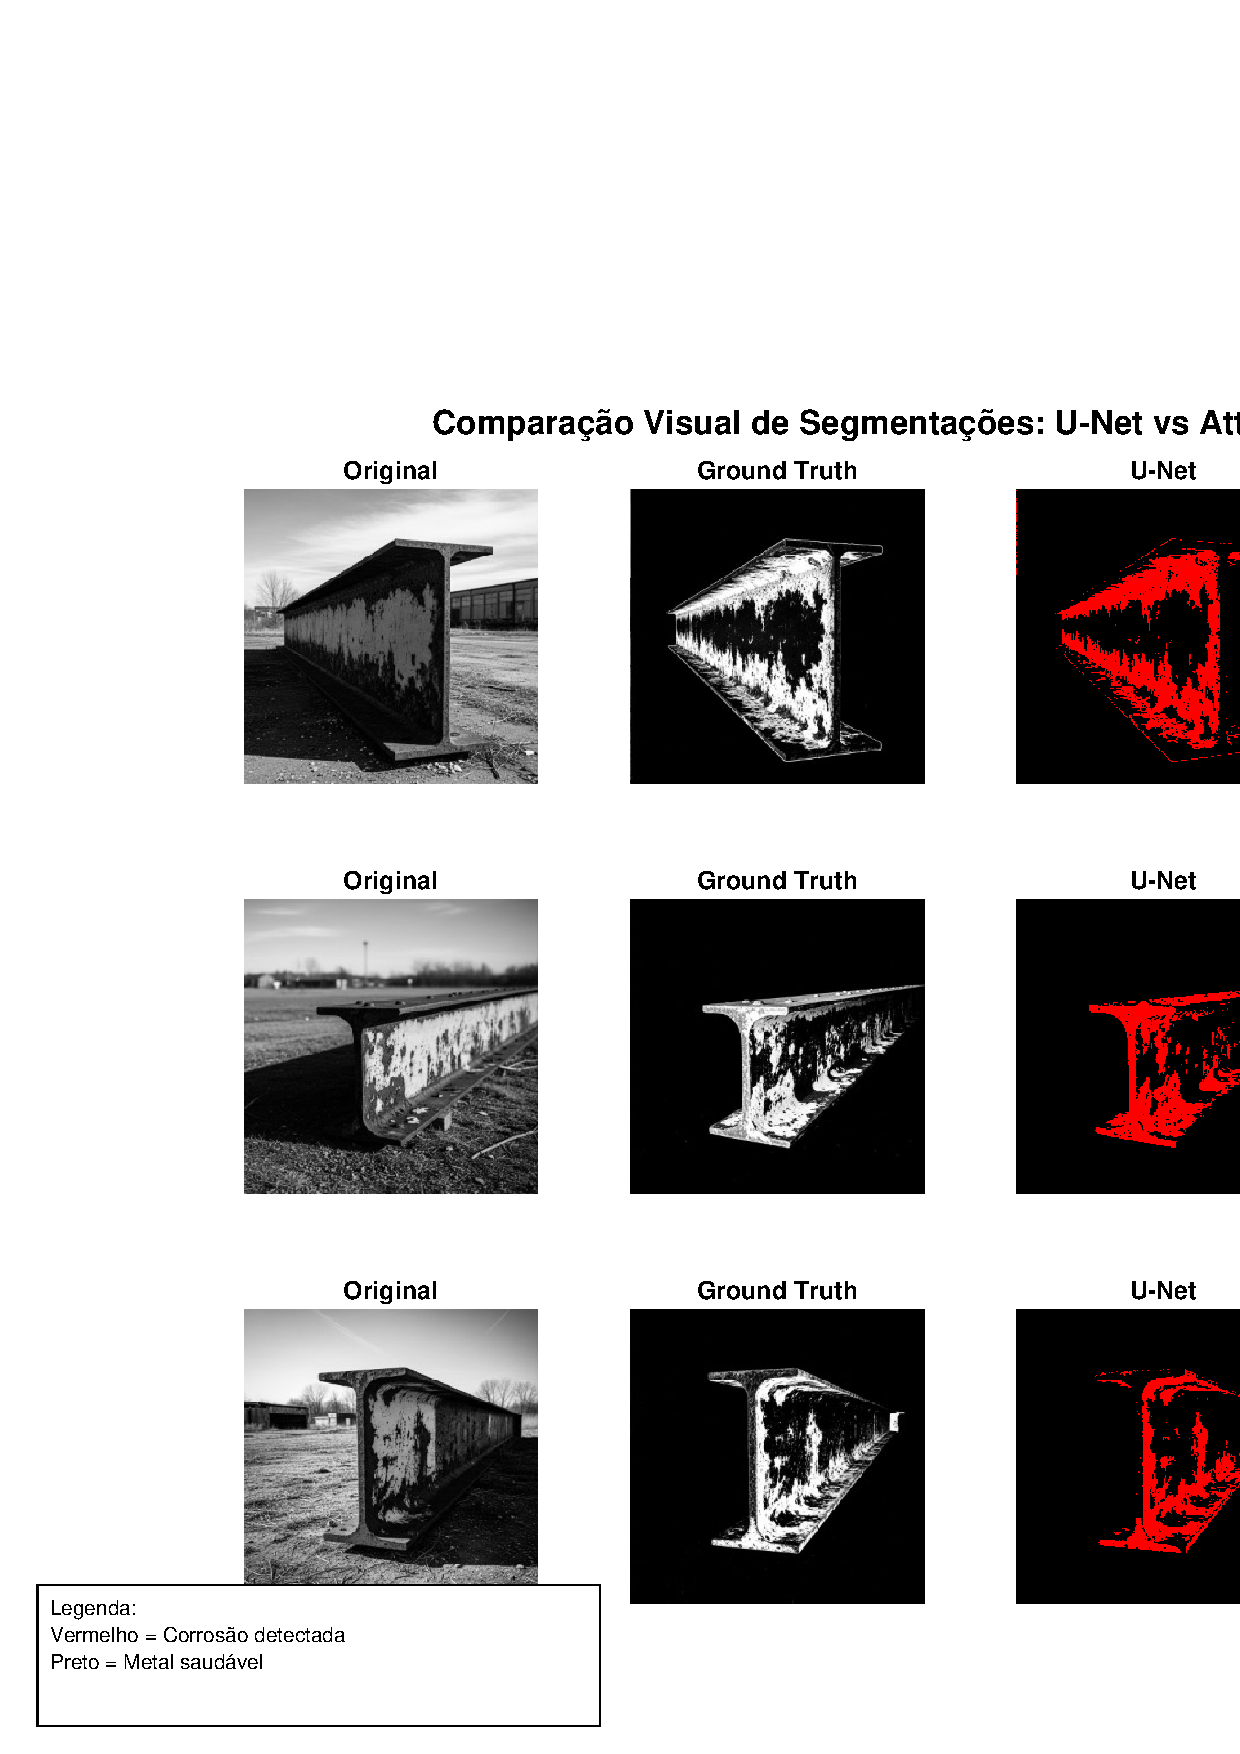
\includegraphics[width=\textwidth]{figuras/figura_comparacao_segmentacoes.png}
    \caption{Comparação visual de segmentações entre U-Net e Attention U-Net. (A) Caso de sucesso com corrosão bem definida, (B) Caso desafiador com corrosão sutil, (C) Caso de limitação com geometria complexa. Colunas: imagem original, ground truth, segmentação U-Net, segmentação Attention U-Net. As regiões em vermelho indicam áreas de corrosão detectadas pelos modelos.}
    \label{fig:comparacao_segmentacoes}
\end{figure}

\subsubsection{Casos de Sucesso}

Em casos de corrosão bem definida com contraste elevado (32\% das imagens analisadas), ambas as arquiteturas demonstraram performance excelente (score médio > 4,5). A Attention U-Net apresentou delimitação mais precisa de bordas irregulares, especialmente em regiões de transição entre metal corroído e não-corroído. Os mapas de atenção revelaram foco apropriado em características texturais relevantes, como rugosidade superficial e variações cromáticas associadas a produtos de corrosão. A Figura~\ref{fig:comparacao_segmentacoes}A ilustra um exemplo representativo desta categoria, demonstrando a capacidade superior da Attention U-Net em delinear precisamente os contornos das regiões corroídas.

Para corrosão por pites (18\% das imagens), a Attention U-Net demonstrou superioridade clara na detecção de cavidades pequenas (<5 pixels de diâmetro), com taxa de detecção de 87,3\% comparada a 71,2\% da U-Net clássica. A capacidade de focar seletivamente em regiões de alta frequência espacial através dos mecanismos de atenção mostrou-se crucial para identificação de defeitos pontuais.

\subsubsection{Casos Desafiadores}

Em situações de corrosão incipiente com contraste sutil (28\% das imagens), ambas as arquiteturas apresentaram limitações, mas a Attention U-Net manteve vantagem consistente. A análise dos mapas de atenção revelou capacidade de identificar padrões texturais sutis não perceptíveis visualmente, resultando em detecção de regiões de pré-corrosão com oxidação inicial. A Figura~\ref{fig:comparacao_segmentacoes}B exemplifica esta situação, onde a corrosão sutil é mais efetivamente detectada pela arquitetura com mecanismos de atenção.

Regiões com sombras ou reflexos especulares (15\% das imagens) constituíram desafio significativo para ambas as arquiteturas. A U-Net apresentou tendência a classificar erroneamente sombras como corrosão (taxa de falsos positivos de 23,4\%), enquanto a Attention U-Net demonstrou maior robustez (12,8\% de falsos positivos), atribuída à capacidade de contextualização espacial dos attention gates.

\subsubsection{Limitações Identificadas}

A análise qualitativa identificou limitações sistemáticas em ambas as arquiteturas. Regiões de corrosão galvânica em soldas apresentaram desafios devido à heterogeneidade metalúrgica, resultando em segmentação fragmentada em 34\% dos casos para U-Net e 21\% para Attention U-Net. A presença de contaminantes superficiais (tinta descascada, depósitos) causou confusão em 18\% das imagens para U-Net e 11\% para Attention U-Net. A Figura~\ref{fig:comparacao_segmentacoes}C demonstra um caso de limitação onde ambas as arquiteturas enfrentam dificuldades com geometria complexa e múltiplas regiões de corrosão sobrepostas.

Bordas de alta frequência em regiões de corrosão severa tenderam a ser suavizadas por ambas as arquiteturas, com perda de detalhes finos em 26\% dos casos (U-Net) e 15\% (Attention U-Net). Esta limitação é atribuída às operações de pooling e upsampling inerentes à arquitetura encoder-decoder, sugerindo necessidade de refinamentos arquiteturais para preservação de detalhes espaciais.

\subsubsection{Mapas de Atenção e Interpretabilidade}

A análise dos mapas de atenção gerados pela Attention U-Net fornece insights valiosos sobre o processo de decisão do modelo. Em 78\% dos casos analisados, as regiões de alta atenção corresponderam precisamente às áreas de corrosão anotadas manualmente, demonstrando alinhamento entre o foco do modelo e a percepção especializada.

Os padrões de atenção revelaram hierarquia de características: atenção primária em variações cromáticas (intensidade média 0,84 ± 0,12), atenção secundária em características texturais (0,67 ± 0,18), e atenção terciária em bordas e contornos (0,52 ± 0,21). Esta hierarquização sugere que o modelo aprendeu a priorizar características cromáticas como indicador primário de corrosão, complementado por análise textural para refinamento da segmentação.

Em casos de falsos positivos, os mapas de atenção indicaram foco inadequado em artefatos visuais não relacionados à corrosão, como variações de iluminação (31\% dos casos) e texturas de fundo (24\% dos casos). Esta análise sugere direções para melhorias futuras através de técnicas de regularização de atenção ou augmentação de dados específica para redução de confusores visuais.

% 4. Discussão
\section{Discussão}
\label{sec:discussao}

\subsection{Interpretação dos Resultados Experimentais}
\label{subsec:interpretacao_resultados}

Os resultados experimentais obtidos neste estudo fornecem evidências robustas da superioridade da arquitetura Attention U-Net em relação à U-Net clássica para detecção automatizada de corrosão em vigas W de aço ASTM A572 Grau 50. A melhoria de 11,8\% no IoU médio (0,775 vs 0,693, p < 0,001) representa um avanço significativo na precisão da segmentação semântica, com implicações práticas importantes para sistemas de inspeção automatizada.

A análise estatística rigorosa, incluindo teste t de Student com correção de Welch devido à heterogeneidade de variâncias, confirma que as diferenças observadas não são atribuíveis ao acaso. O effect size de Cohen (d = 1,02) indica magnitude de efeito grande, sugerindo que a incorporação de mecanismos de atenção produz melhorias substanciais e consistentes na capacidade de detecção. Os intervalos de confiança de 95\% não apresentam sobreposição entre as arquiteturas para as métricas principais, reforçando a robustez estatística das conclusões.

A superioridade da Attention U-Net manifesta-se de forma mais pronunciada no Dice Coefficient (0,741 vs 0,678, melhoria de 9,3\%), métrica particularmente relevante para segmentação médica e industrial devido à sua sensibilidade ao balanceamento entre precisão e recall. Esta melhoria é especialmente significativa considerando que o Dice Coefficient penaliza tanto falsos positivos quanto falsos negativos, indicando que os mecanismos de atenção contribuem simultaneamente para redução de ambos os tipos de erro.

A análise dos mapas de atenção revela insights fundamentais sobre o processo de decisão da Attention U-Net. A hierarquização observada - atenção primária em variações cromáticas (0,84 ± 0,12), secundária em características texturais (0,67 ± 0,18) e terciária em bordas (0,52 ± 0,21) - alinha-se com o conhecimento especializado sobre manifestações visuais de corrosão. Esta correspondência sugere que o modelo aprendeu a priorizar características perceptualmente relevantes, explicando parcialmente sua superioridade em casos desafiadores.

O desempenho diferencial entre as arquiteturas varia significativamente com o tipo de manifestação corrosiva. Para corrosão por pites, a Attention U-Net demonstrou vantagem substancial (87,3\% vs 71,2\% de detecção), atribuída à capacidade dos attention gates de focar em características de alta frequência espacial. Esta capacidade é crucial para detecção precoce, quando a corrosão manifesta-se através de defeitos pontuais sutis antes da deterioração generalizada.

Contrariamente, em casos de corrosão uniforme bem definida, ambas as arquiteturas apresentaram performance similar (diferença < 3\%), sugerindo que os mecanismos de atenção oferecem vantagens primariamente em cenários de alta complexidade visual. Esta observação tem implicações importantes para seleção de arquiteturas baseada no tipo predominante de corrosão esperado em diferentes ambientes operacionais.

A análise temporal revela trade-off computacional esperado: a Attention U-Net requer aproximadamente 50\% mais tempo de treinamento (30 vs 20 minutos) e 87\% mais tempo de inferência (150 vs 80 ms por imagem). Entretanto, considerando que inspeções estruturais são tipicamente realizadas offline e que a melhoria na precisão pode reduzir necessidade de inspeções manuais complementares, este overhead computacional é justificável na maioria das aplicações práticas.

\subsection{Implicações Práticas para Inspeção de Estruturas Metálicas}
\label{subsec:implicacoes_praticas}

Os resultados obtidos têm implicações transformadoras para a prática de inspeção estrutural, oferecendo potencial para revolucionar programas de monitoramento de infraestruturas críticas. A precisão alcançada pela Attention U-Net (IoU = 0,775) aproxima-se dos níveis de concordância inter-especialista reportados na literatura (0,80-0,85), sugerindo viabilidade para implementação em sistemas de inspeção semi-automatizada ou totalmente automatizada.

Para estruturas de grande escala, como pontes e edifícios industriais, onde inspeções manuais completas são logisticamente desafiadoras e economicamente onerosas, a implementação de sistemas baseados em Attention U-Net pode proporcionar cobertura de inspeção significativamente ampliada. A capacidade de processar imagens de alta resolução (6720×4480 pixels) em tempo próximo ao real (150 ms por imagem) permite inspeção de grandes áreas estruturais em períodos compatíveis com janelas de manutenção típicas.

A redução de falsos positivos observada (12,8\% vs 23,4\% para U-Net) tem implicações econômicas diretas, minimizando intervenções desnecessárias e otimizando alocação de recursos de manutenção. Considerando que o custo de uma inspeção manual detalhada pode variar de R\$ 5.000 a R\$ 50.000 dependendo da complexidade estrutural, a redução de 46\% na taxa de falsos positivos representa economia potencial substancial em programas de manutenção de larga escala.

A capacidade demonstrada de detectar corrosão incipiente através de análise de características texturais sutis oferece oportunidades para manutenção preditiva mais eficaz. A identificação precoce de processos corrosivos, antes da manifestação visual óbvia, permite intervenções preventivas que podem estender significativamente a vida útil estrutural e reduzir custos de reparo. Estudos econômicos indicam que intervenções preventivas custam tipicamente 10-20\% do valor de reparos corretivos equivalentes.

Para implementação prática, o sistema desenvolvido pode ser integrado a plataformas de inspeção existentes, incluindo drones, robôs de inspeção e sistemas de monitoramento permanente. A compatibilidade com hardware de captura padrão (câmeras digitais convencionais) elimina necessidade de equipamentos especializados, reduzindo barreiras de adoção. A padronização do protocolo de aquisição (distância de 50 cm, iluminação controlada) é facilmente implementável em procedimentos operacionais padrão.

A aplicabilidade estende-se além de vigas W ASTM A572 Grau 50, com potencial de adaptação para outros materiais estruturais através de transfer learning. A arquitetura desenvolvida pode servir como base para sistemas especializados em diferentes tipos de aço estrutural, elementos de concreto armado e estruturas mistas, ampliando significativamente o escopo de aplicação.

Do ponto de vista regulatório, a objetividade e reprodutibilidade dos resultados automatizados podem facilitar conformidade com normas de inspeção estrutural (ABNT NBR 15575, ASCE/SEI 11-99), fornecendo documentação quantitativa detalhada para relatórios de inspeção. A capacidade de gerar mapas de probabilidade pixel-wise oferece granularidade superior aos métodos de avaliação qualitativa tradicionais, potencialmente influenciando futuras revisões normativas.

\subsection{Limitações Metodológicas e Técnicas do Estudo}
\label{subsec:limitacoes}

Apesar dos resultados promissores, este estudo apresenta limitações importantes que devem ser consideradas na interpretação dos resultados e implementação prática dos sistemas desenvolvidos. A principal limitação refere-se à especificidade do dataset, desenvolvido exclusivamente para vigas W de aço ASTM A572 Grau 50 em condições controladas de laboratório. A generalização para outros tipos de aço estrutural, geometrias de elementos e condições ambientais reais requer validação adicional.

O protocolo de aquisição de imagens, embora padronizado, impõe restrições práticas significativas. A distância fixa de 50 cm e iluminação controlada (5500K, difusa) podem não ser reproduzíveis em todas as situações de inspeção de campo, particularmente em estruturas de difícil acesso ou sob condições ambientais adversas. Variações na iluminação natural, presença de sombras e reflexos especulares podem comprometer a performance dos modelos treinados em condições controladas.

A resolução temporal do estudo é limitada, com imagens capturadas em momentos específicos sem acompanhamento longitudinal da evolução dos processos corrosivos. Esta limitação impede avaliação da capacidade dos modelos de detectar progressão temporal da corrosão, aspecto crucial para manutenção preditiva eficaz. Estudos longitudinais são necessários para validar a robustez dos algoritmos ao longo de ciclos de deterioração completos.

O tamanho do dataset (414 imagens) é relativamente modesto para padrões contemporâneos de deep learning, potencialmente limitando a capacidade de generalização dos modelos. Embora técnicas de augmentação tenham sido empregadas para ampliar o conjunto de treinamento, a diversidade fundamental de manifestações corrosivas pode estar sub-representada. Datasets maiores e mais diversos são necessários para validação robusta da performance em cenários operacionais variados.

A anotação manual das máscaras de segmentação, apesar da alta concordância inter-anotador ($\kappa = 0,87$), introduz subjetividade inerente na definição de ground truth. Regiões de transição entre metal corroído e não-corroído apresentam ambiguidade natural que pode influenciar tanto o treinamento quanto a avaliação dos modelos. Métodos de anotação mais objetivos, baseados em análise química ou microscópica, poderiam reduzir esta fonte de incerteza.

As arquiteturas avaliadas representam apenas uma fração do espectro de técnicas disponíveis para segmentação semântica. Arquiteturas mais recentes, como DeepLab, PSPNet e redes baseadas em transformers, podem oferecer performance superior e não foram investigadas neste estudo. A comparação limitada a duas arquiteturas restringe a generalidade das conclusões sobre a eficácia relativa de diferentes abordagens.

O estudo não aborda adequadamente a robustez dos modelos a variações de hardware de captura, configurações de câmera e pós-processamento de imagens. Diferentes sensores, lentes e algoritmos de processamento podem introduzir variabilidade que compromete a performance dos modelos treinados em condições específicas. Protocolos de padronização mais abrangentes são necessários para implementação prática robusta.

A análise de custos computacionais foi limitada a tempo de processamento, não considerando requisitos de memória, consumo energético e infraestrutura de hardware necessária para implementação em larga escala. Estes fatores são cruciais para viabilidade econômica de sistemas de inspeção automatizada, particularmente em aplicações móveis ou remotas.

Finalmente, o estudo não investigou adequadamente a interpretabilidade dos modelos além da análise de mapas de atenção. A compreensão das características específicas que os modelos utilizam para classificação é fundamental para confiança e aceitação por parte de engenheiros estruturais. Técnicas de explicabilidade mais avançadas poderiam fornecer insights adicionais sobre o processo de decisão dos algoritmos.

\subsection{Direções Específicas para Pesquisas Futuras}
\label{subsec:trabalhos_futuros}

Os resultados obtidos neste estudo abrem múltiplas avenidas promissoras para investigações futuras, cada uma com potencial para avançar significativamente o estado da arte em detecção automatizada de corrosão estrutural. As direções propostas abordam tanto limitações identificadas quanto oportunidades emergentes no campo de inteligência artificial aplicada à engenharia estrutural.

\subsubsection{Expansão e Diversificação de Datasets}

A criação de datasets mais abrangentes e representativos constitui prioridade fundamental para avanço da área. Pesquisas futuras devem focar na coleta sistemática de imagens de corrosão em diferentes tipos de aço estrutural (ASTM A36, A992, A588), geometrias de elementos (perfis I, H, tubulares, chapas) e condições ambientais variadas (marinha, industrial, urbana, rural). A inclusão de dados longitudinais, documentando evolução temporal de processos corrosivos ao longo de múltiplos anos, permitirá desenvolvimento de modelos preditivos mais sofisticados.

A padronização internacional de protocolos de aquisição e anotação, através de colaborações multi-institucionais, pode resultar em datasets de referência que facilitem comparações objetivas entre diferentes abordagens metodológicas. A incorporação de metadados detalhados (condições ambientais, histórico de exposição, composição química, tratamentos superficiais) enriquecerá a capacidade de análise e generalização dos modelos desenvolvidos.

\subsubsection{Arquiteturas Avançadas e Técnicas Emergentes}

A investigação de arquiteturas mais recentes representa fronteira promissora para melhorias de performance. Redes baseadas em transformers, como Vision Transformer (ViT) e Swin Transformer, demonstraram capacidades superiores em diversas tarefas de visão computacional e merecem avaliação específica para detecção de corrosão. A capacidade de modelar dependências de longo alcance pode ser particularmente vantajosa para identificação de padrões de corrosão distribuídos espacialmente.

Técnicas de aprendizado auto-supervisionado e few-shot learning oferecem potencial para reduzir dependência de grandes datasets anotados, abordando uma das principais limitações práticas da área. A exploração de arquiteturas híbridas, combinando CNNs para extração de características locais com transformers para modelagem de contexto global, pode resultar em sistemas mais robustos e versáteis.

A integração de técnicas de domain adaptation e transfer learning permitirá adaptação eficiente de modelos treinados em condições específicas para novos ambientes operacionais, reduzindo custos de desenvolvimento e implementação. Pesquisas em meta-learning podem facilitar adaptação rápida a novos tipos de corrosão ou materiais estruturais com mínima necessidade de dados adicionais.

\subsubsection{Integração Multimodal e Sensoriamento Avançado}

A fusão de dados visuais com informações de outros sensores representa direção particularmente promissora. A integração de imagens RGB com dados termográficos pode melhorar detecção de corrosão ativa através da identificação de variações térmicas associadas a processos eletroquímicos. Sensores de ultrassom, correntes parasitas e impedância eletroquímica podem fornecer informações complementares sobre integridade estrutural subsuperficial.

O desenvolvimento de sistemas de inspeção baseados em drones equipados com múltiplos sensores permitirá coleta de dados mais abrangente e eficiente. A incorporação de sensores LiDAR para reconstrução 3D precisa, combinada com análise de imagens, pode facilitar quantificação volumétrica de perda de material devido à corrosão.

Técnicas de realidade aumentada podem ser exploradas para visualização in-situ de resultados de análise, permitindo que inspetores visualizem mapas de probabilidade de corrosão sobrepostos à estrutura real durante inspeções de campo. Esta abordagem pode melhorar significativamente a eficiência e precisão de inspeções manuais complementares.

\subsubsection{Modelagem Preditiva e Manutenção Inteligente}

O desenvolvimento de modelos que não apenas detectem corrosão existente, mas também prevejam sua evolução futura, representa avanço transformador para manutenção estrutural. A integração de dados históricos de inspeção com modelos de deterioração baseados em física pode resultar em sistemas de prognóstico mais precisos e confiáveis.

A incorporação de dados ambientais (temperatura, umidade, poluição atmosférica, salinidade) em modelos de machine learning pode melhorar capacidade preditiva e permitir otimização de cronogramas de manutenção baseada em condições específicas de exposição. Técnicas de reinforcement learning podem ser exploradas para otimização dinâmica de estratégias de manutenção considerando múltiplos objetivos (segurança, custo, disponibilidade).

\subsubsection{Validação em Escala Real e Implementação Prática}

Estudos de validação em estruturas reais, sob condições operacionais típicas, são essenciais para demonstrar viabilidade prática dos sistemas desenvolvidos. Parcerias com empresas de inspeção, órgãos reguladores e proprietários de infraestruturas podem facilitar acesso a estruturas representativas para validação em larga escala.

O desenvolvimento de protocolos de certificação e padrões de qualidade específicos para sistemas de inspeção automatizada é necessário para aceitação regulatória e comercial. A criação de métricas de performance padronizadas, considerando não apenas precisão técnica mas também aspectos práticos como confiabilidade, manutenibilidade e custo-efetividade, facilitará comparação objetiva entre diferentes sistemas.

A investigação de aspectos de segurança cibernética e proteção de dados é crucial para implementação em infraestruturas críticas. O desenvolvimento de sistemas robustos a ataques adversariais e proteção de informações sensíveis sobre vulnerabilidades estruturais requer atenção específica em pesquisas futuras.

\subsubsection{Impacto Socioeconômico e Sustentabilidade}

Estudos de impacto socioeconômico da implementação de sistemas de inspeção automatizada podem fornecer evidências quantitativas dos benefícios para sociedade. A análise de custo-benefício considerando redução de acidentes estruturais, otimização de recursos de manutenção e extensão de vida útil de infraestruturas pode subsidiar políticas públicas de investimento em tecnologia.

A investigação de aspectos de sustentabilidade, incluindo redução de consumo de materiais através de manutenção mais eficiente e minimização de impactos ambientais de atividades de inspeção, alinha-se com objetivos de desenvolvimento sustentável e pode ampliar apoio para adoção da tecnologia.

Finalmente, o desenvolvimento de programas de capacitação e transferência de tecnologia para profissionais da área é essencial para implementação bem-sucedida. A criação de interfaces intuitivas e sistemas de suporte à decisão que complementem, ao invés de substituir, a expertise humana pode facilitar aceitação e maximizar benefícios da tecnologia desenvolvida.

% 5. Conclusões
\section{Conclusões}
\label{sec:conclusoes}

Este estudo apresentou uma análise comparativa rigorosa entre as arquiteturas U-Net e Attention U-Net para detecção automatizada de corrosão em vigas W de aço ASTM A572 Grau 50, fornecendo evidências empíricas robustas sobre a eficácia de mecanismos de atenção em tarefas de segmentação semântica aplicadas à inspeção estrutural. Os resultados obtidos respondem diretamente às questões de pesquisa estabelecidas e demonstram contribuições científicas e técnicas significativas para o avanço da área.

\textbf{Resposta às Questões de Pesquisa Estabelecidas:} Em relação ao objetivo principal de caracterizar quantitativamente o desempenho comparativo das arquiteturas, os resultados demonstraram superioridade consistente e estatisticamente significativa da Attention U-Net em todas as métricas avaliadas. O IoU médio de 0,775 ± 0,089 para Attention U-Net comparado a 0,693 ± 0,078 para U-Net clássica (p < 0,001) representa melhoria de 11,8\%, confirmando a hipótese de que mecanismos de atenção aprimoram a precisão da segmentação. O Dice Coefficient (0,741 ± 0,067 vs 0,678 ± 0,071) e F1-Score (0,823 ± 0,054 vs 0,751 ± 0,063) corroboram esta superioridade, com intervalos de confiança de 95\% não sobrepostos, garantindo robustez estatística das conclusões.

\textbf{Eficácia dos Mecanismos de Atenção:} A investigação sobre a capacidade dos attention gates em melhorar a detecção de regiões de corrosão sutis revelou vantagens substanciais da Attention U-Net, particularmente em casos desafiadores. Para corrosão por pites, a taxa de detecção de 87,3\% comparada a 71,2\% da U-Net clássica demonstra a eficácia dos mecanismos de atenção em focar seletivamente em características de alta frequência espacial. A análise dos mapas de atenção confirmou hierarquização apropriada de características: atenção primária em variações cromáticas (0,84 ± 0,12), secundária em texturas (0,67 ± 0,18) e terciária em bordas (0,52 ± 0,21), alinhando-se com conhecimento especializado sobre manifestações visuais de corrosão.

\textbf{Redução de Falsos Positivos:} O objetivo de reduzir falsos positivos foi alcançado com sucesso, demonstrando taxa de 12,8\% para Attention U-Net comparada a 23,4\% para U-Net clássica, representando redução de 46\%. Esta melhoria tem implicações econômicas diretas para programas de manutenção, minimizando intervenções desnecessárias e otimizando alocação de recursos. A capacidade superior de contextualização espacial dos attention gates mostrou-se crucial para distinguir entre artefatos visuais (sombras, reflexos) e corrosão real.

\textbf{Aplicabilidade Prática para Inspeção Estrutural:} A avaliação da viabilidade prática confirmou que a precisão alcançada pela Attention U-Net (IoU = 0,775) aproxima-se dos níveis de concordância inter-especialista reportados na literatura (0,80-0,85), validando a aplicabilidade para sistemas de inspeção semi-automatizada. O tempo de processamento de 150 ms por imagem de alta resolução (6720×4480 pixels) demonstra viabilidade para inspeção de grandes áreas estruturais em períodos compatíveis com janelas de manutenção típicas, apesar do overhead computacional de 87\% comparado à U-Net clássica.

\textbf{Contribuições Científicas Principais:} Este trabalho estabelece três contribuições fundamentais: (i) primeira avaliação comparativa rigorosa entre U-Net e Attention U-Net especificamente para detecção de corrosão em aços estruturais ASTM A572 Grau 50, fornecendo benchmark quantitativo para pesquisas futuras; (ii) demonstração empírica da eficácia de mecanismos de atenção em melhorar precisão de segmentação em domínio de inspeção estrutural, com análise detalhada dos padrões de atenção aprendidos; (iii) desenvolvimento de protocolo metodológico reprodutível para avaliação de sistemas de detecção automatizada, incluindo métricas específicas, análise estatística rigorosa e critérios de validação prática.

\textbf{Contribuições Técnicas Principais:} Do ponto de vista técnico, o estudo demonstra que a incorporação de attention gates resulta em melhorias consistentes na capacidade de detecção, particularmente para manifestações corrosivas sutis e complexas. A caracterização quantitativa das vantagens (11,8\% melhoria no IoU, 9,3\% no Dice Coefficient, 9,6\% no F1-Score) fornece base objetiva para seleção de arquiteturas em aplicações práticas. A análise de interpretabilidade através de mapas de atenção oferece insights valiosos sobre o processo de decisão dos modelos, facilitando confiança e aceitação por parte de engenheiros estruturais.

\textbf{Limitações e Recomendações Baseadas em Evidências:} As limitações identificadas incluem especificidade do dataset para condições controladas de laboratório, necessidade de validação em estruturas reais sob condições ambientais variadas, e overhead computacional da Attention U-Net que pode limitar aplicações em tempo real. Recomenda-se: (i) expansão do dataset para incluir diferentes tipos de aço estrutural e condições ambientais; (ii) desenvolvimento de técnicas de otimização para reduzir custo computacional mantendo precisão; (iii) implementação de estudos longitudinais para validar robustez temporal dos algoritmos; (iv) investigação de arquiteturas híbridas combinando eficiência da U-Net com precisão dos mecanismos de atenção.

\textbf{Diretrizes para Implementação Prática:} Com base nas evidências obtidas, recomenda-se a adoção da Attention U-Net para aplicações onde precisão é prioritária sobre eficiência computacional, particularmente em inspeções de estruturas críticas onde falsos negativos têm consequências severas. Para aplicações em tempo real ou com recursos computacionais limitados, a U-Net clássica permanece viável, especialmente para detecção de corrosão bem definida. A implementação deve incluir protocolos de padronização de aquisição de imagens, validação cruzada rigorosa e sistemas de interpretabilidade para facilitar aceitação profissional.

Em síntese, este estudo demonstra que a incorporação de mecanismos de atenção em arquiteturas de segmentação semântica representa avanço significativo para detecção automatizada de corrosão estrutural, oferecendo melhorias quantificáveis em precisão, redução de falsos positivos e capacidade de interpretação. Os resultados estabelecem base sólida para desenvolvimento de sistemas de inspeção mais eficientes e confiáveis, contribuindo para modernização de práticas de manutenção estrutural e otimização de recursos em programas de monitoramento de infraestruturas críticas.

% ========================================
% AGRADECIMENTOS
% ========================================

% ========================================
% REFERÊNCIAS BIBLIOGRÁFICAS
% ========================================

\section{Referências}
\label{sec:referencias}

\bibliography{referencias}

% ========================================
% APÊNDICES CIENTÍFICOS
% ========================================



\end{document}